
% \begin{frame}{Prioritization Has Limited Impact on Result Arrival Time}
%   \vspace{-0.5cm}
%   \begin{center}
%     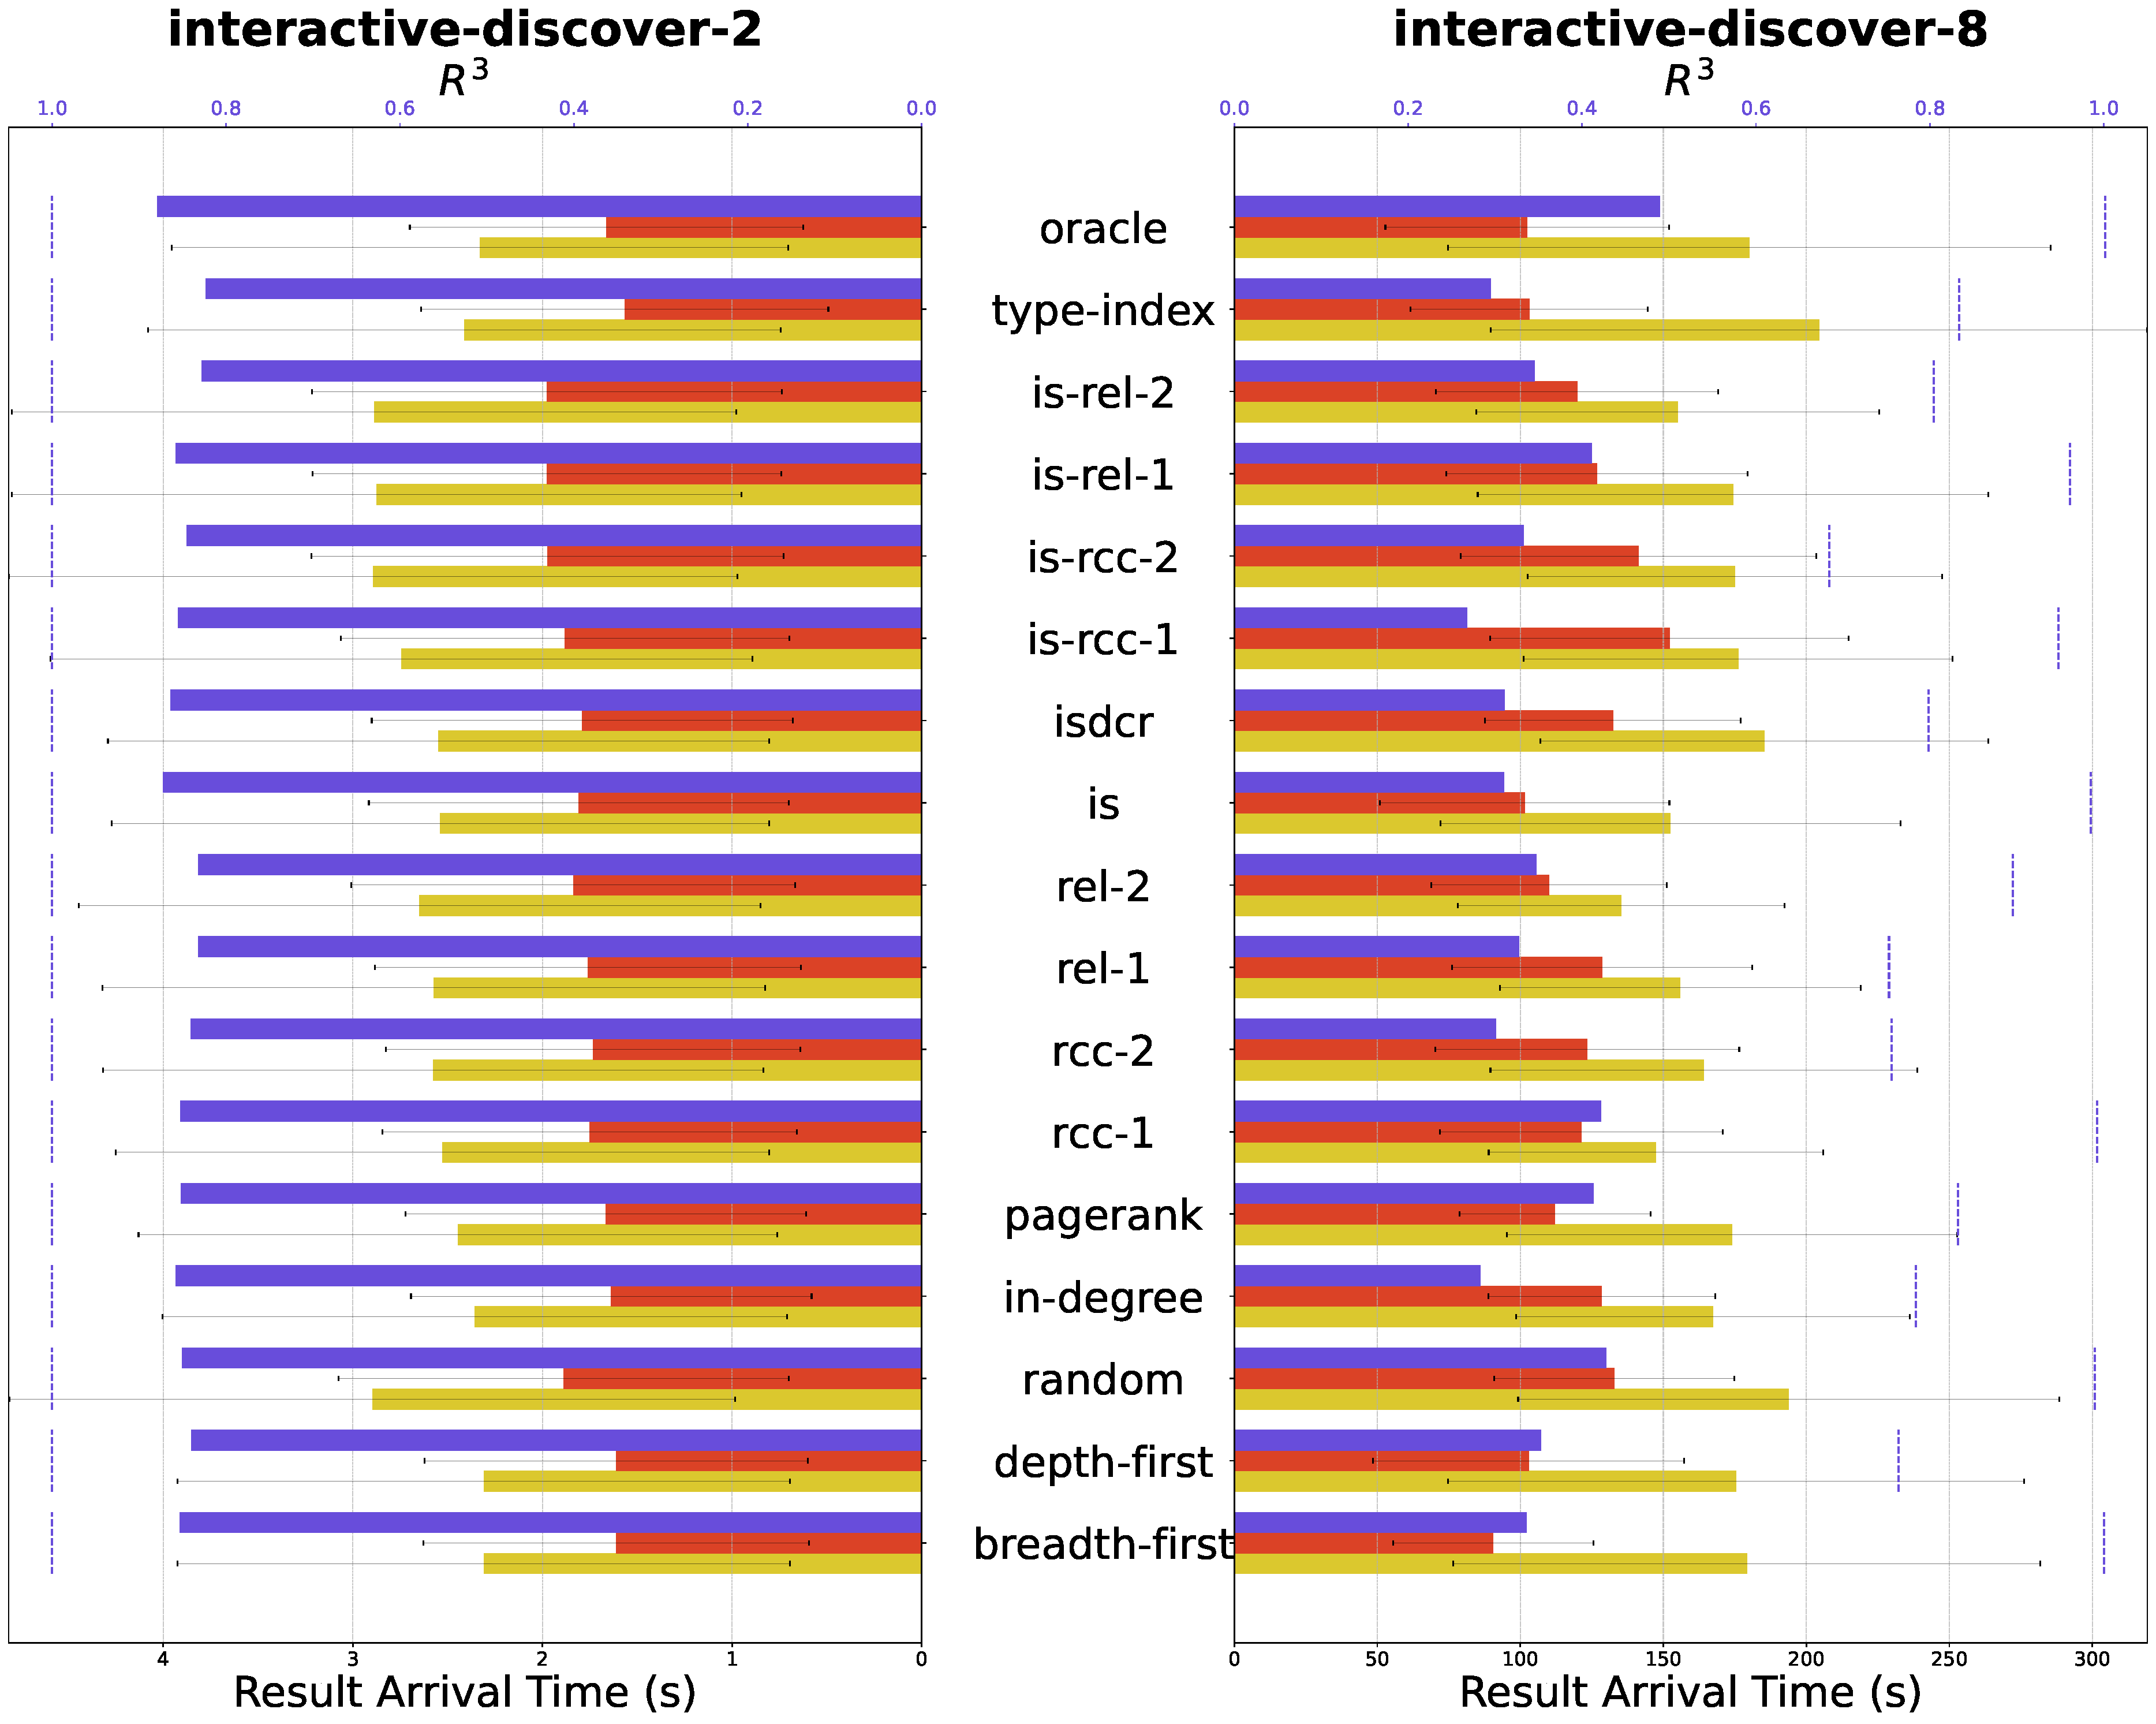
\includegraphics[width=\linewidth,height=0.7\textheight,keepaspectratio]{images/reduced-result-plot-presentation.pdf}
%   \end{center}
%   \vspace{0.3cm}

%   \begin{center}
%     \small
%     \begin{itemize}
%         \item Breadth-first outperforms most algorithms
%         \item Oracle has significantly better $R^{3}$, but not execution time
%     \end{itemize}
%   \end{center}
% \end{frame}

% NOTES: 
%   - FIgure should be entire slide, x / y ticks should be bigger, animation to pop in boxes of text on where to focus and comments on it

% \begin{frame}{Prioritization Has Limited Impact on Result Arrival Time}
%     \begin{columns}[T] % T aligns columns at the top
%         % Left column: Image
%         \begin{column}{0.6\textwidth} % Adjust width as needed
%             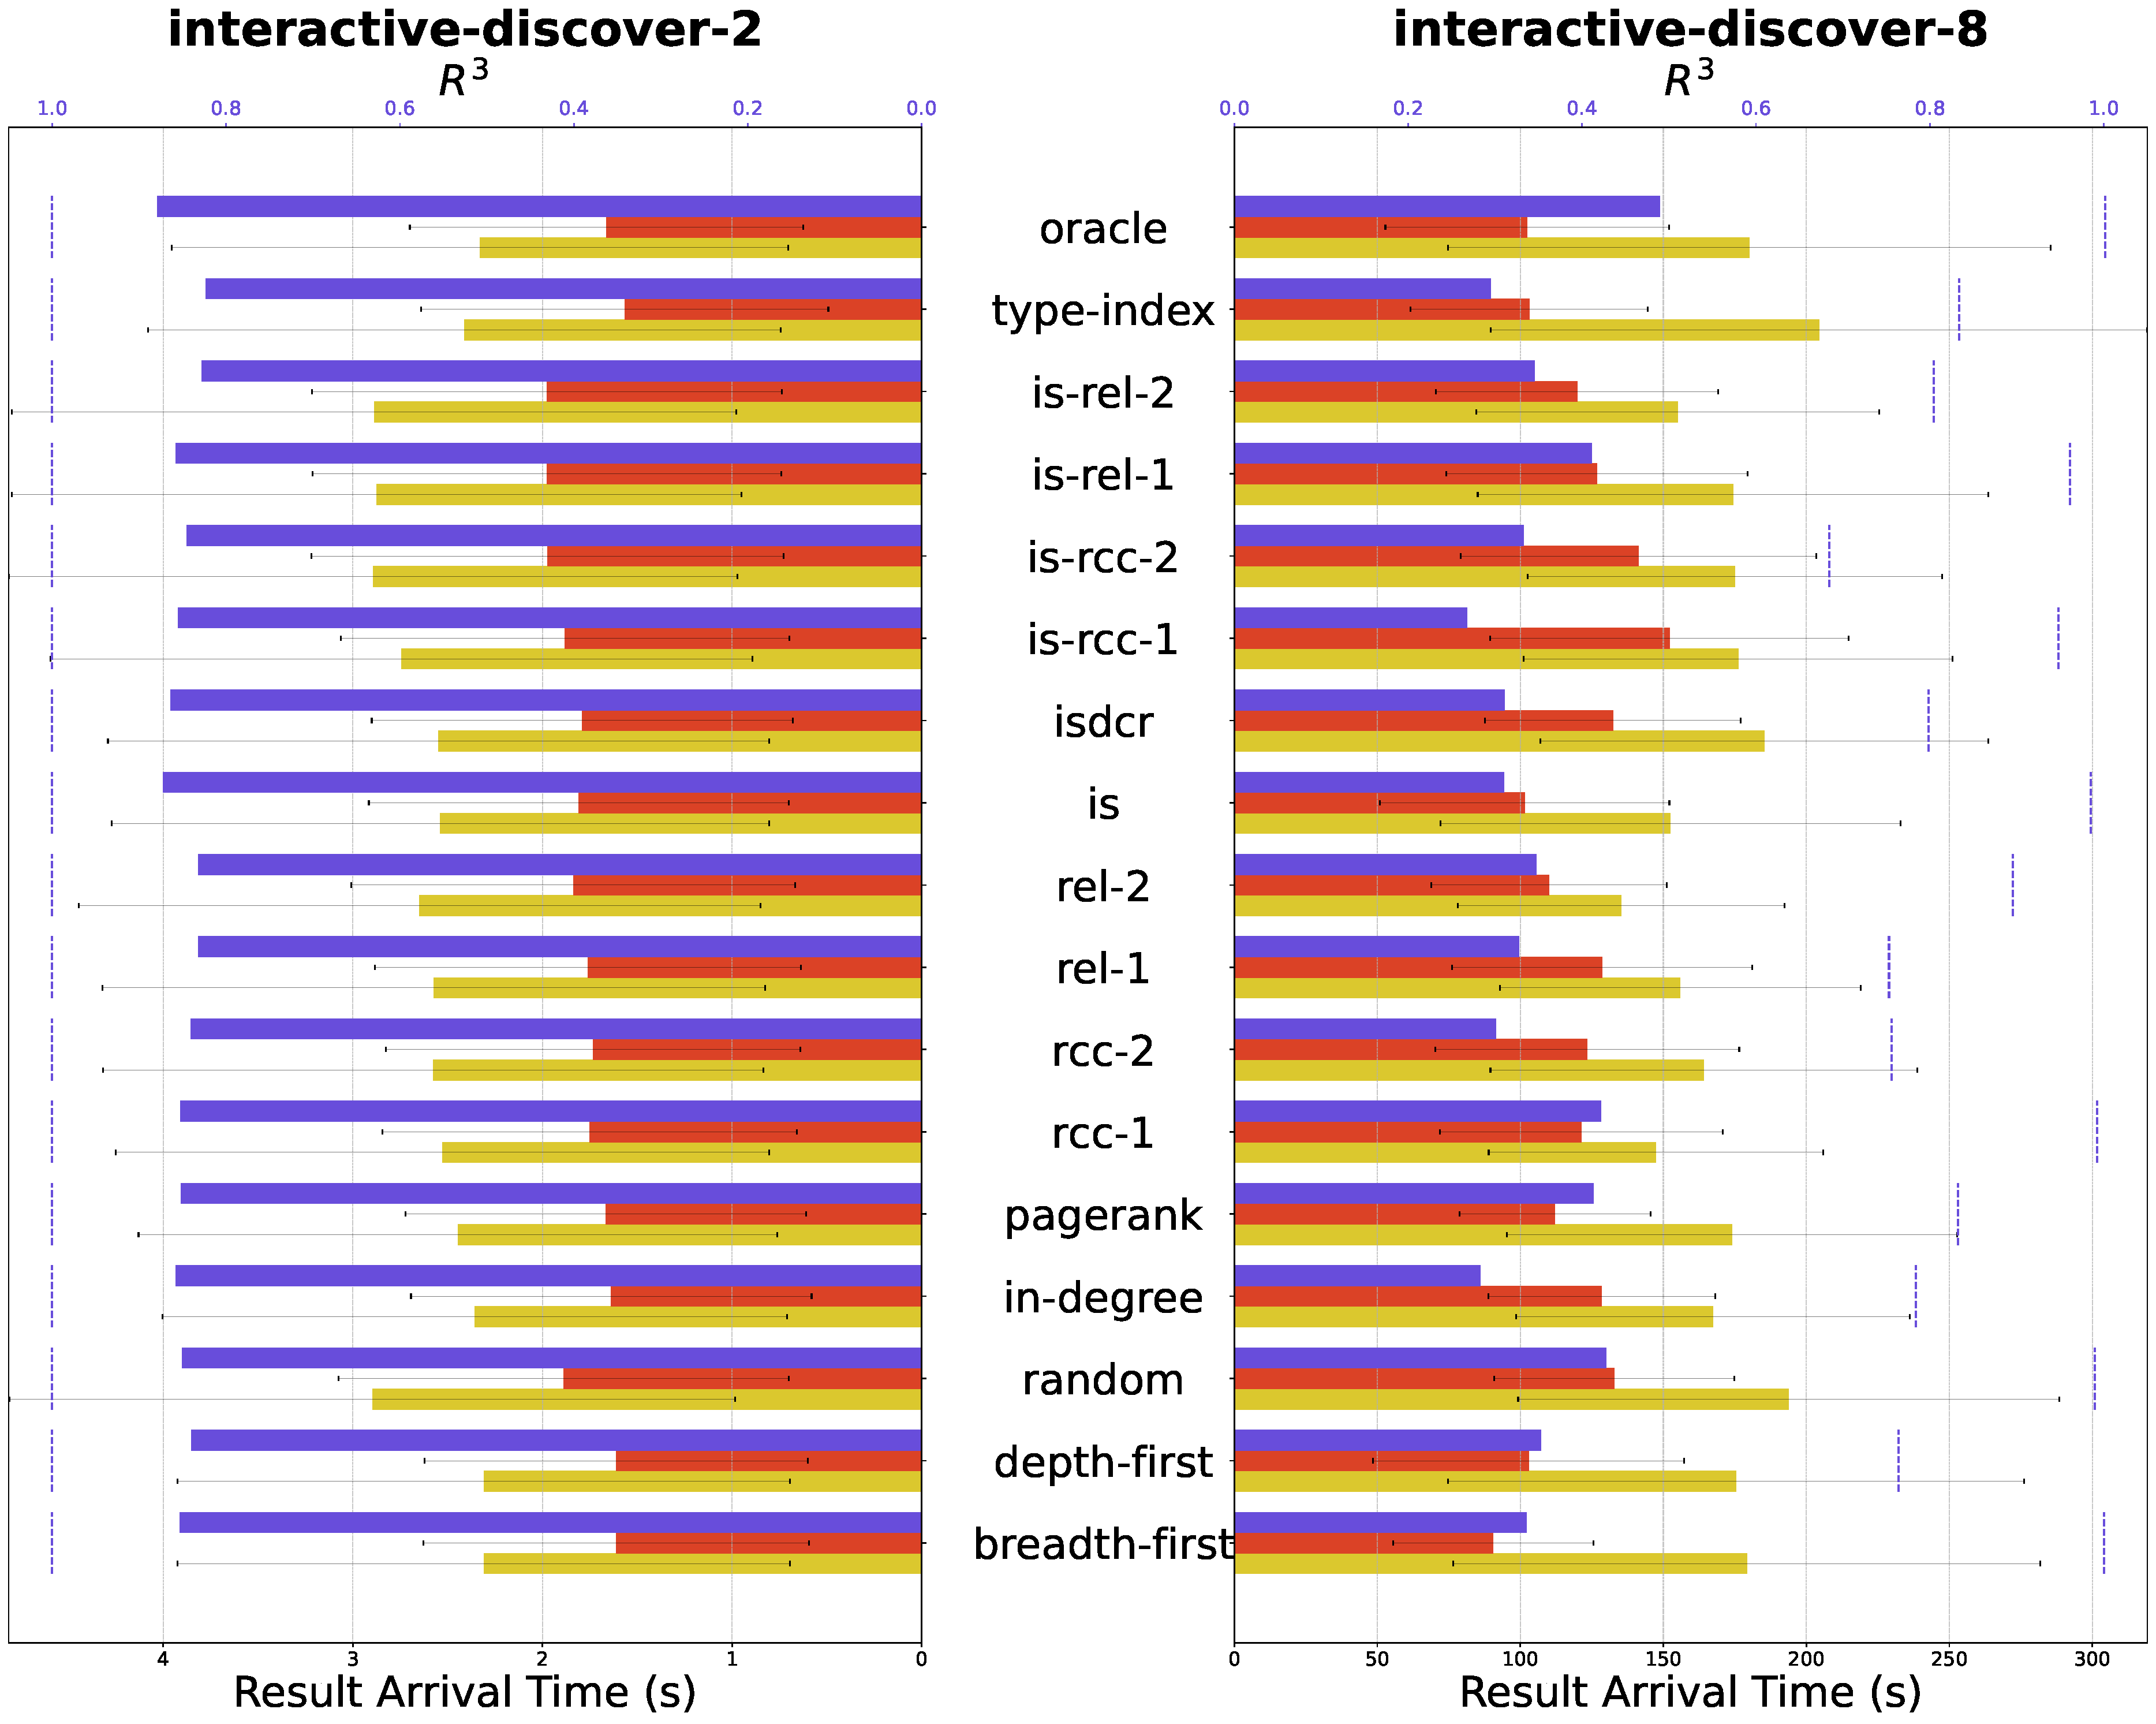
\includegraphics[width=\linewidth]{images/reduced-result-plot-presentation.pdf} % replace with your image file
%         \end{column}

%         % Right column: Text
%         \begin{column}{0.4\textwidth}
%           \begin{itemize}
%               \item Breadth-first outperforms most algorithms
%               \item Oracle has significantly better $R^{3}$, but not execution time
%           \end{itemize}
%         \end{column}
%     \end{columns}
% \end{frame}

\begin{frame}{Prioritization Has Limited Impact on Result Arrival Time}
      \centering
    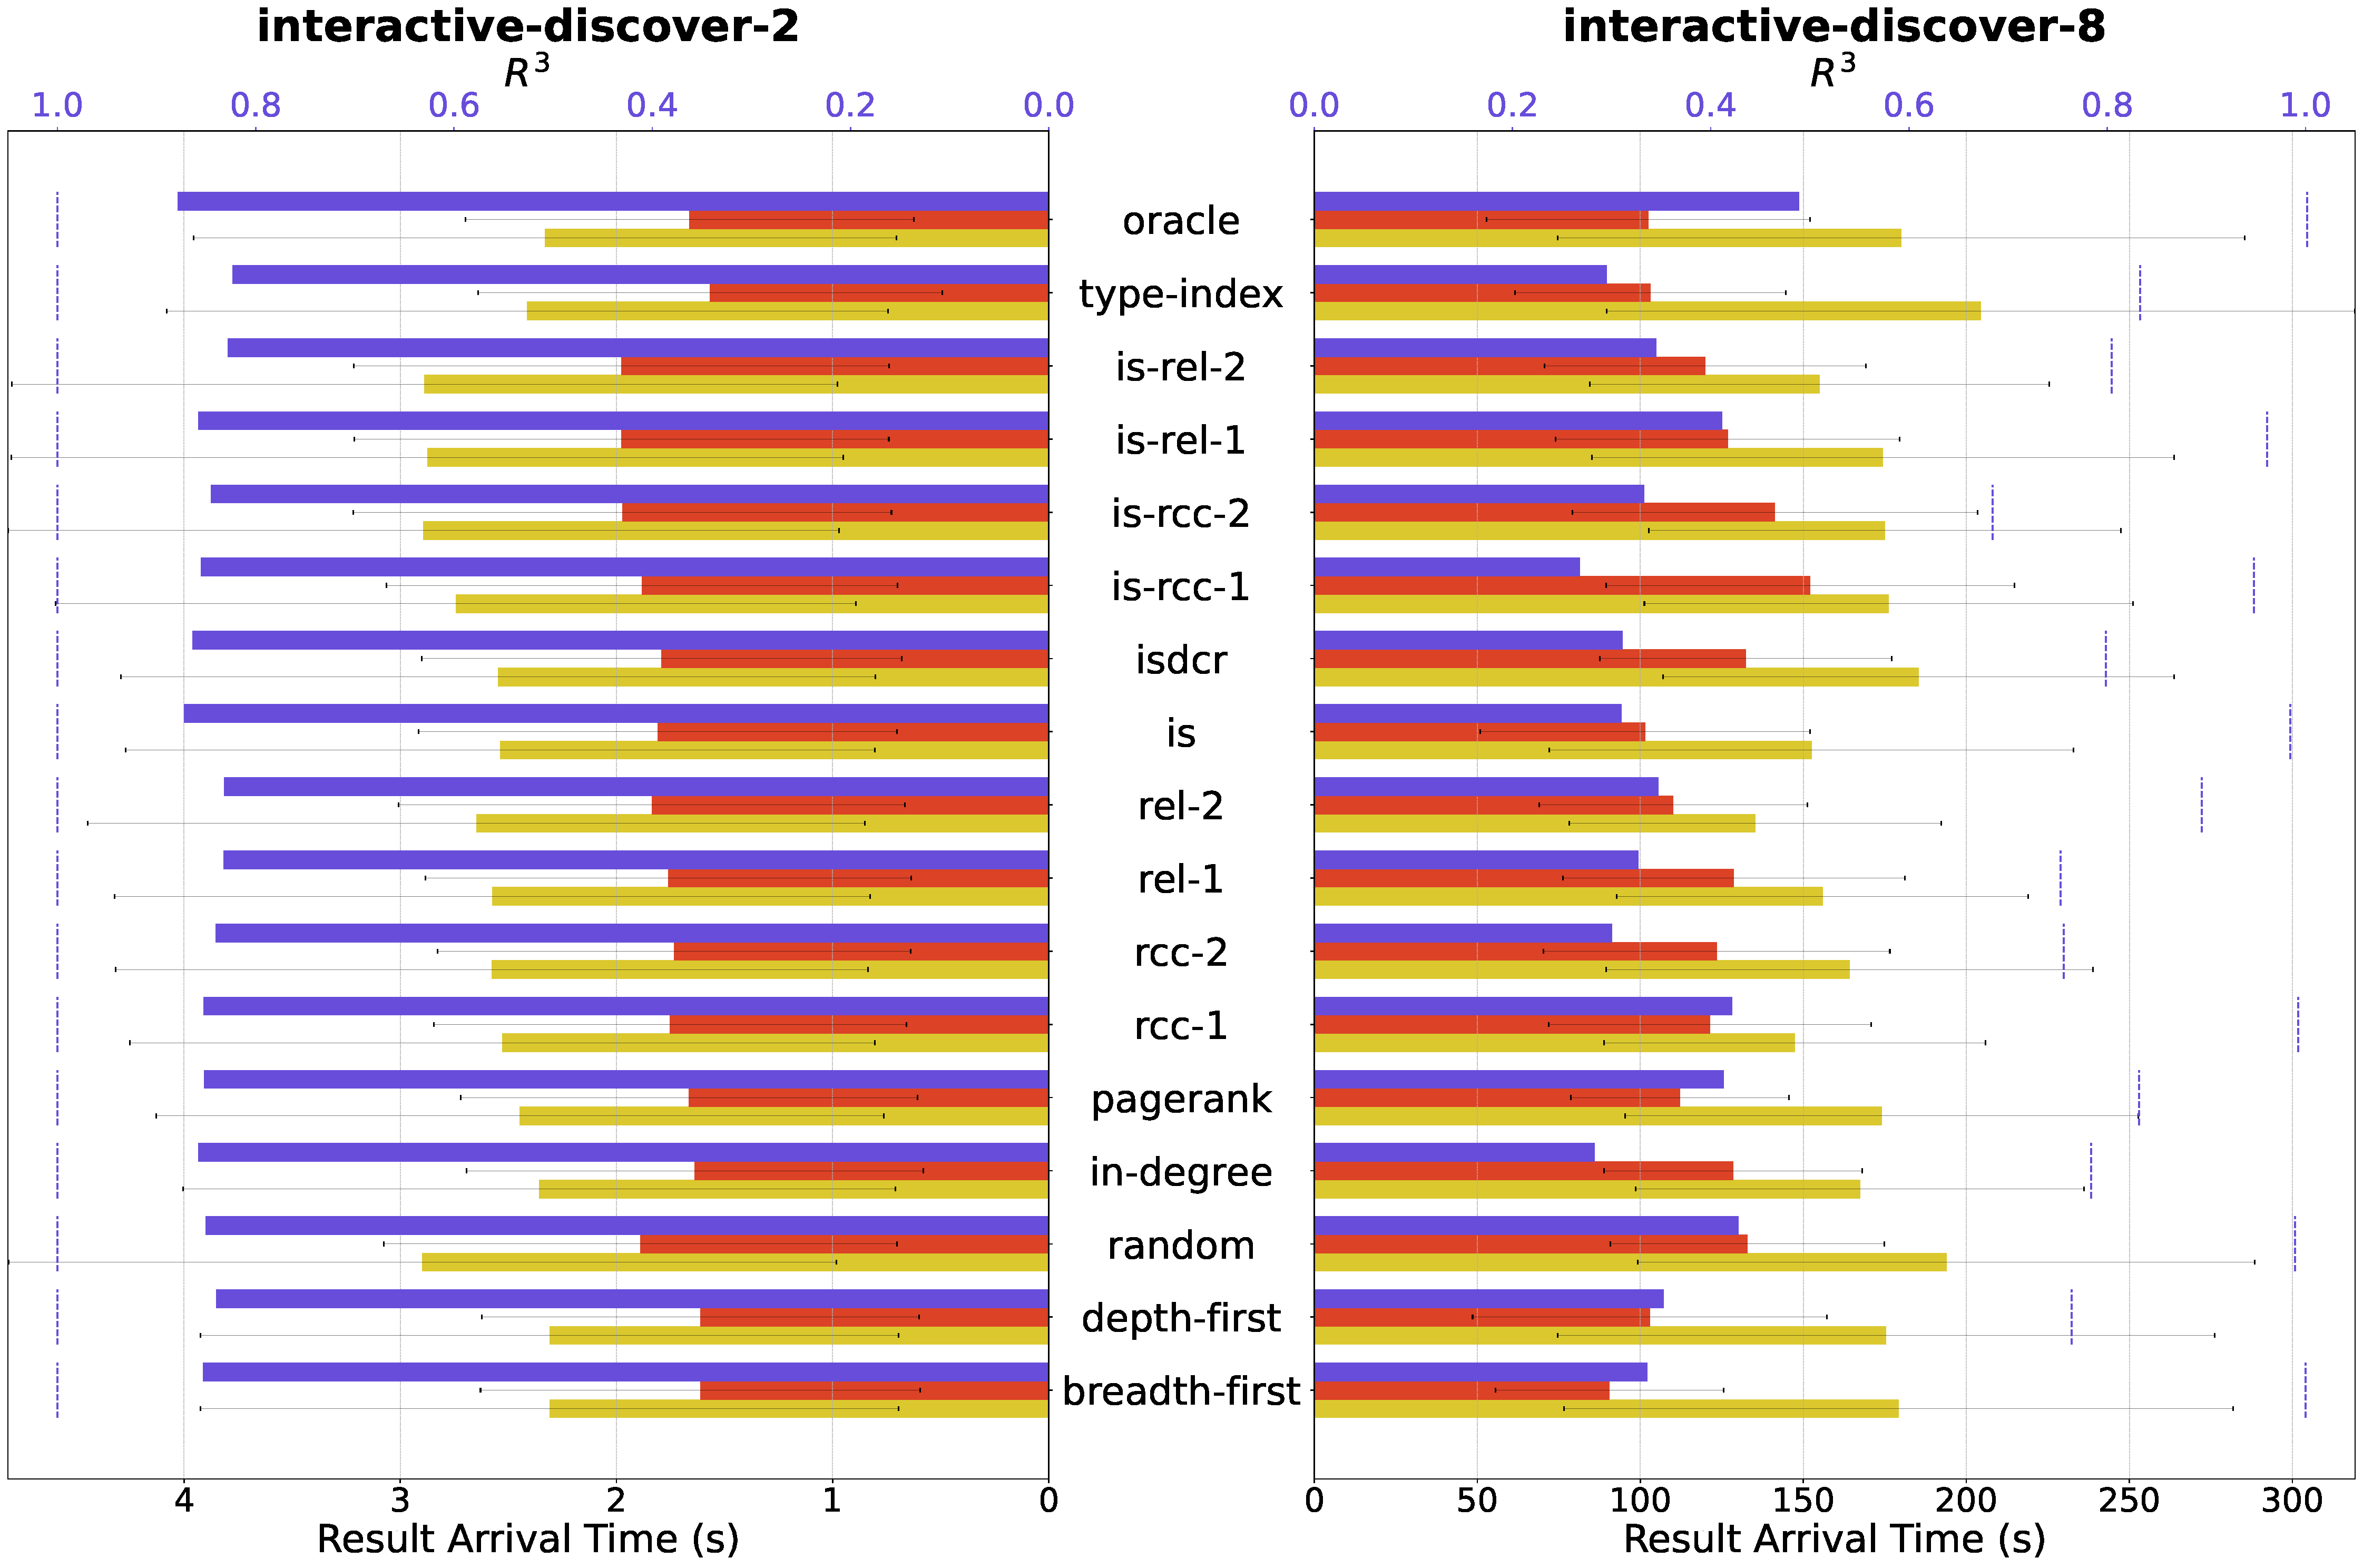
\includegraphics[width=.82\linewidth]{images/combined_r3_timings_plot_non_relative_reduced_test.pdf} % replace with your image file
\end{frame}
\begin{frame}{Prioritization Has Limited Impact on Result Arrival Time}
    \centering
    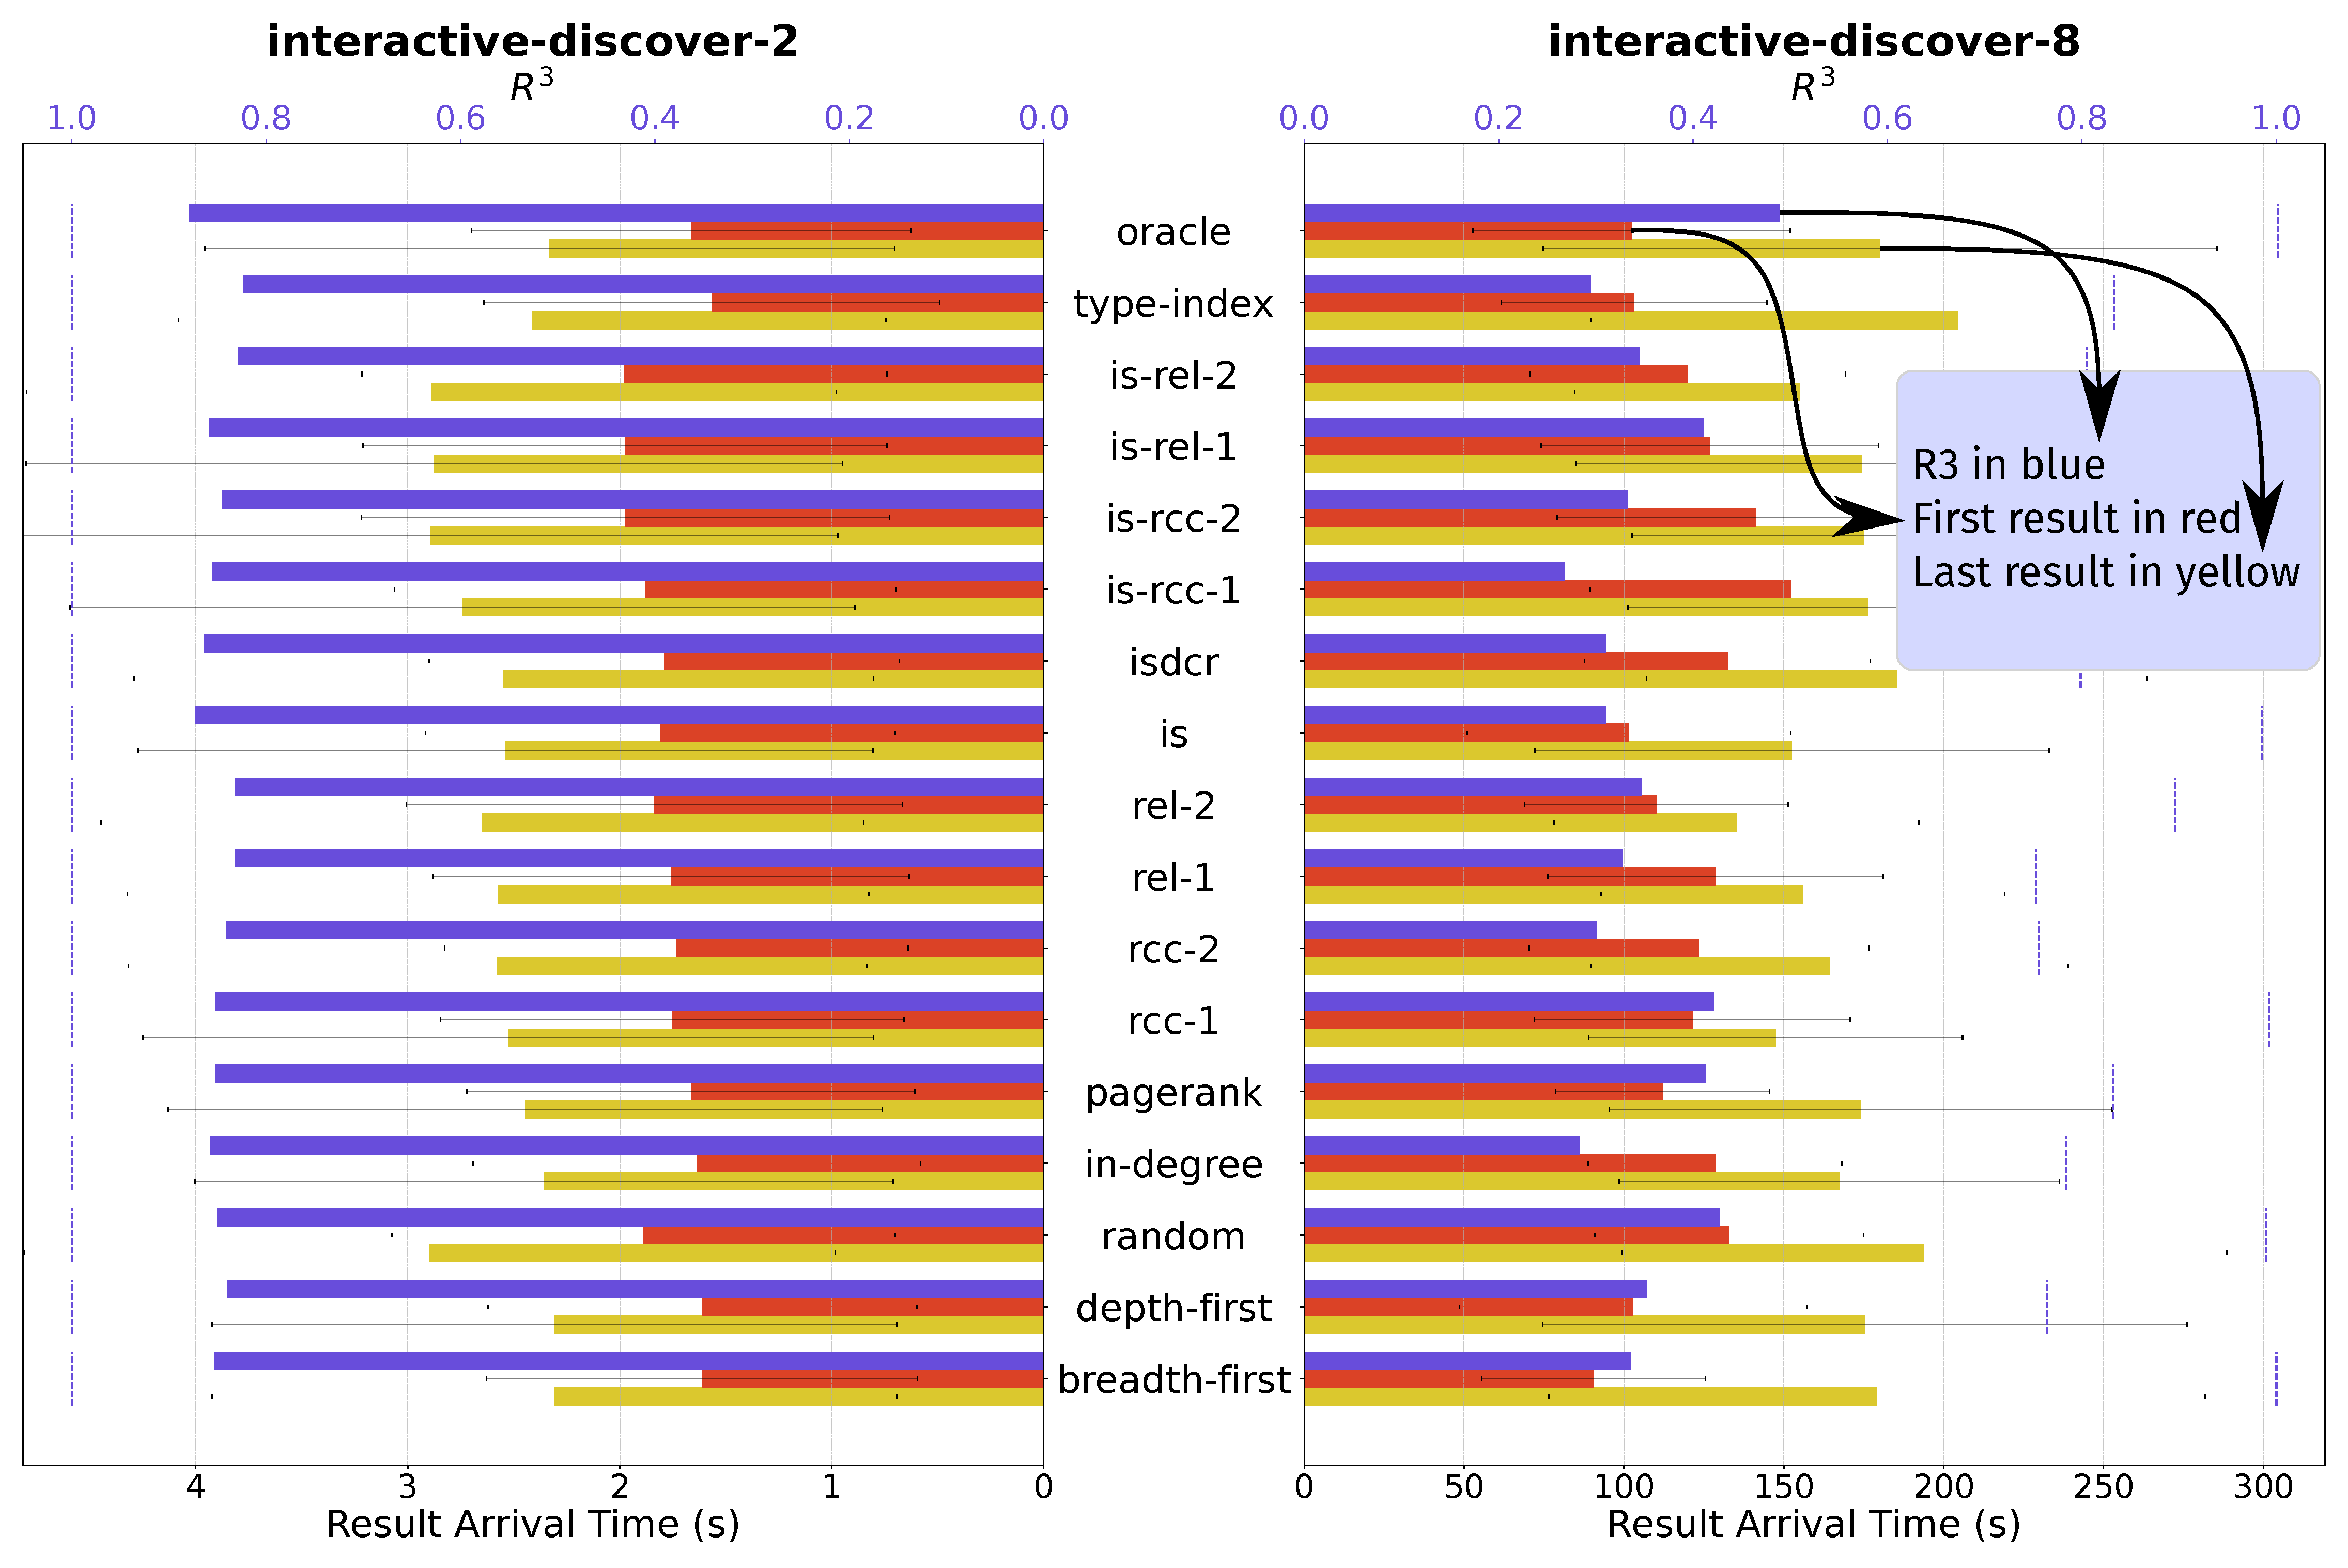
\includegraphics[width=.82\linewidth]{images/plot_color_annotated.pdf} % replace with your image file
\end{frame}
\begin{frame}{Prioritization Has Limited Impact on Result Arrival Time}
    \centering
    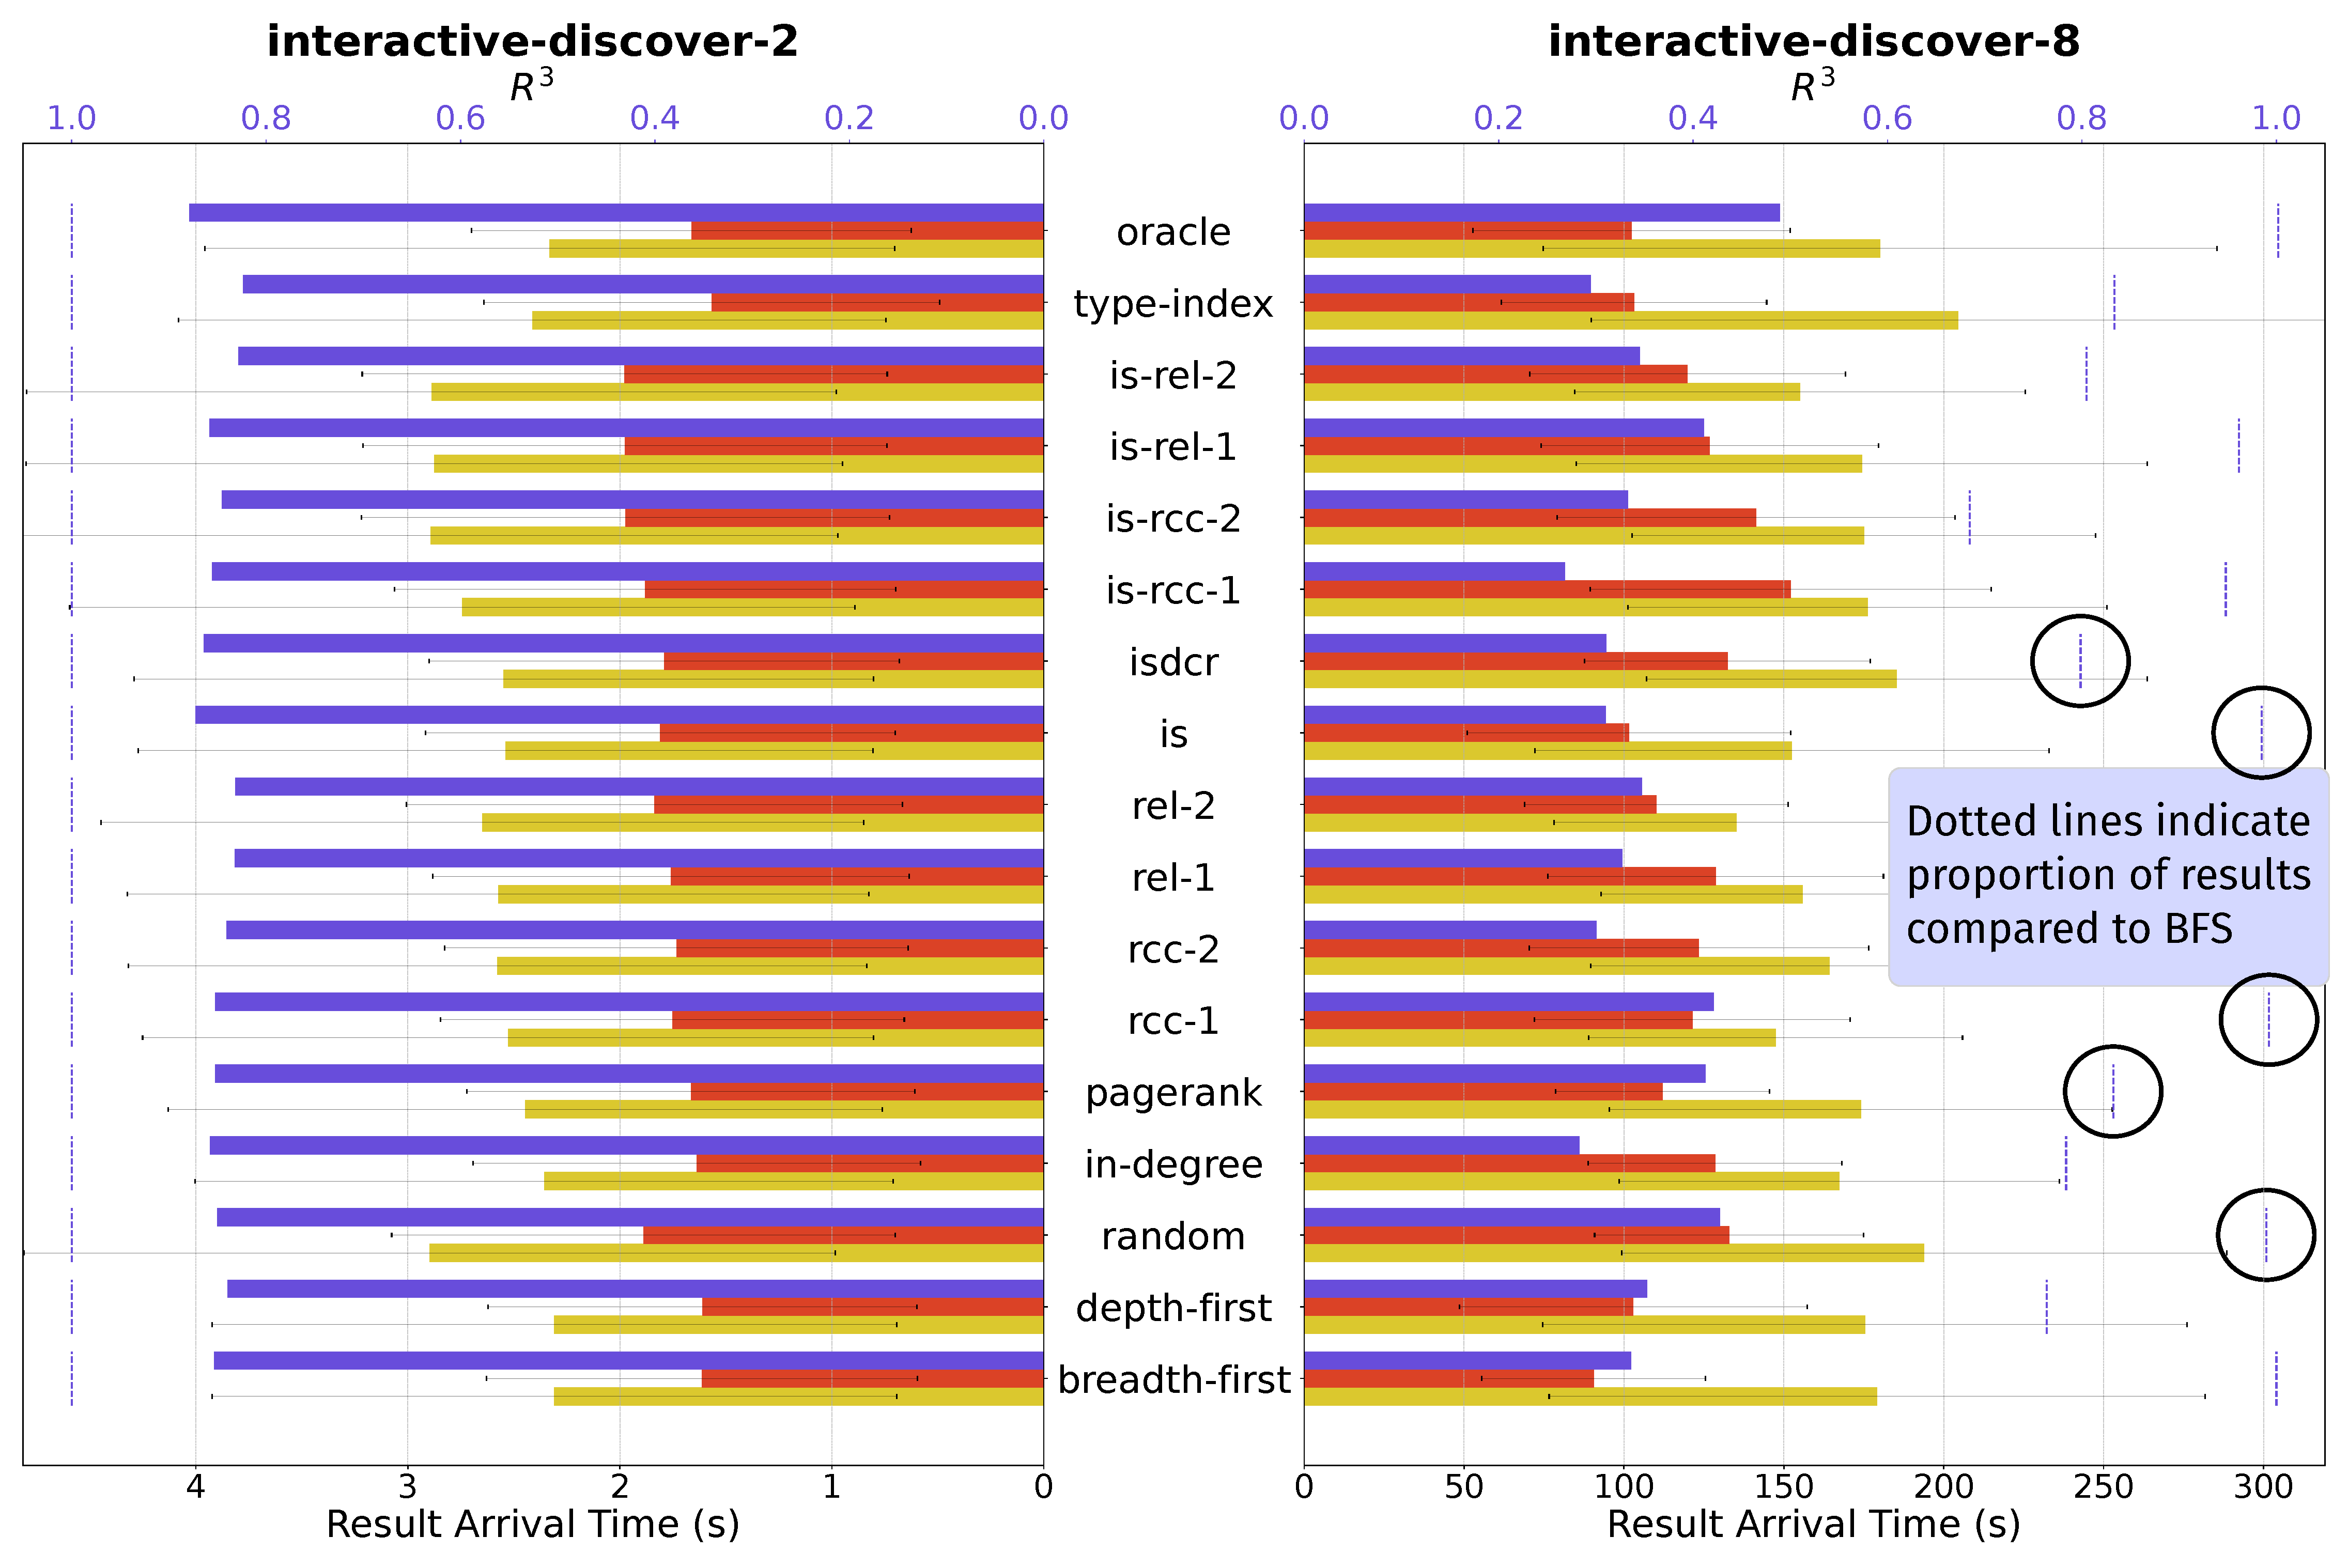
\includegraphics[width=.82\linewidth]{images/plot_dotted_annotated.pdf} % replace with your image file
\end{frame}
\begin{frame}{Prioritization Has Limited Impact on Result Arrival Time}
    \centering
    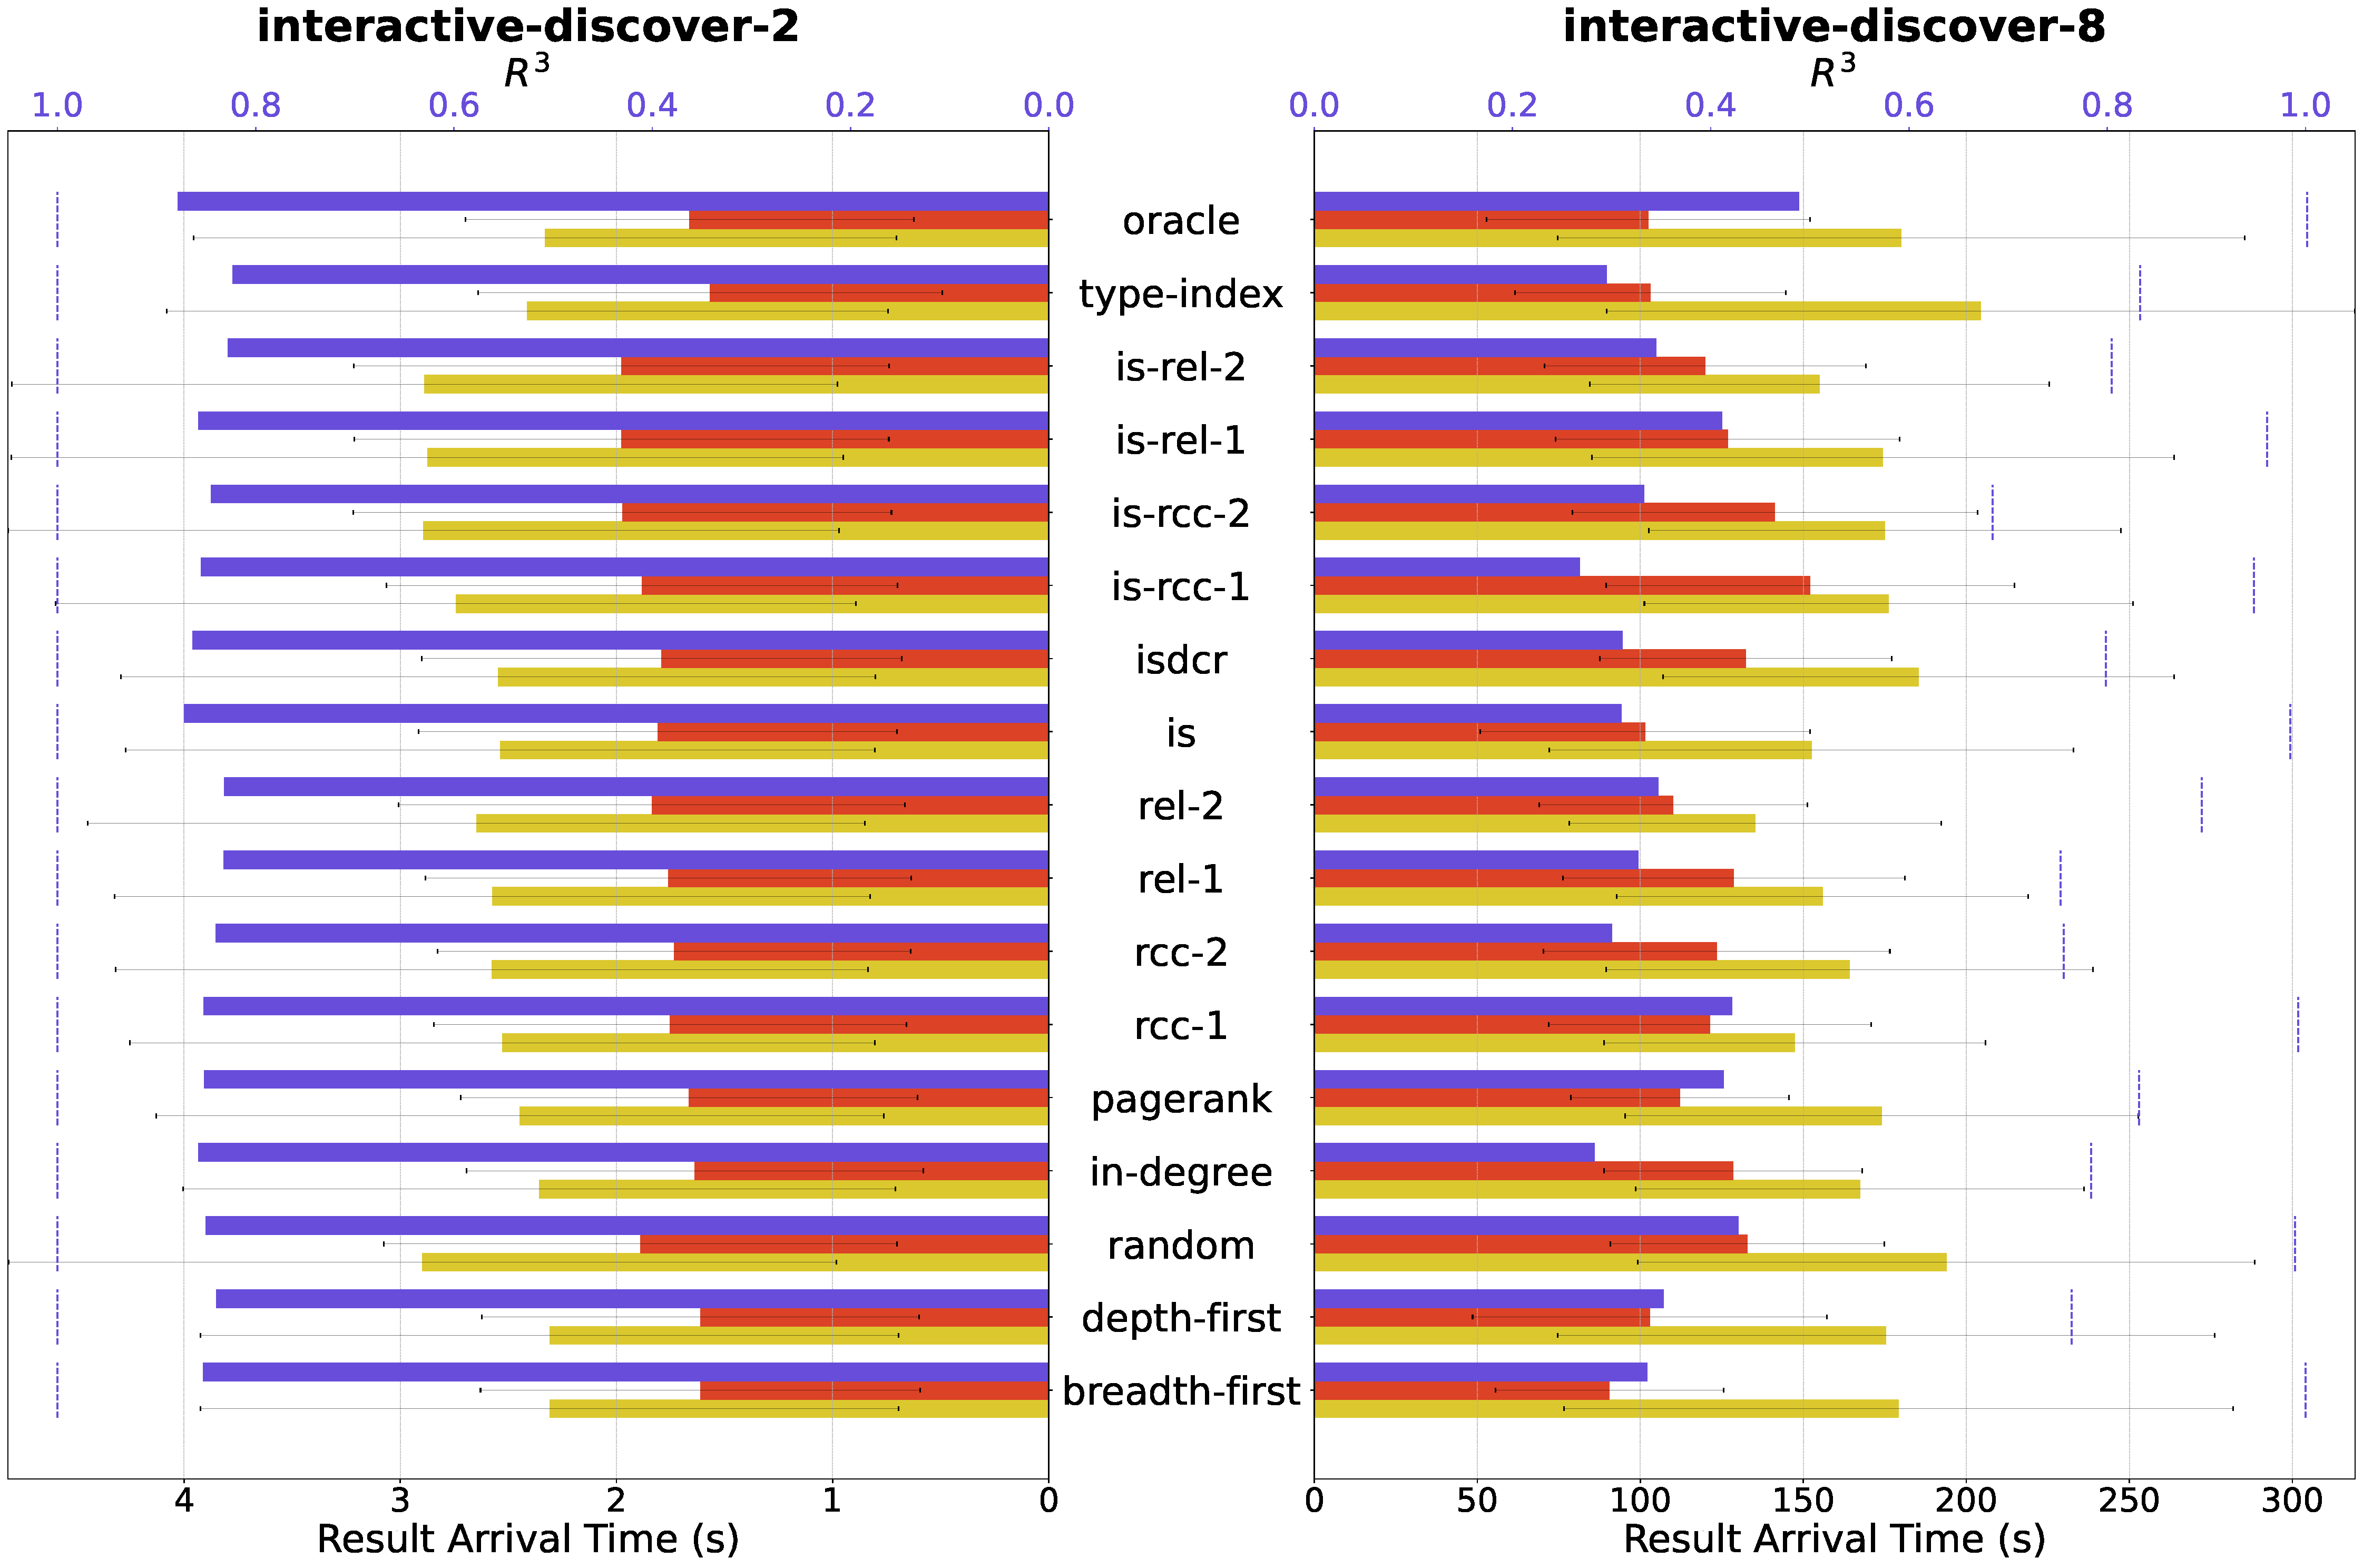
\includegraphics[width=.82\linewidth]{images/combined_r3_timings_plot_non_relative_reduced_test.pdf} % replace with your image file
\end{frame}


\begin{frame}{Prioritization Has Limited Impact on Result Arrival Time}
  \small % or \footnotesize, \scriptsize
  \captionsetup[table]{skip=10pt, font=footnotesize }
  \begin{table}[!ht]
    \centering
    \begin{adjustbox}{width=0.9\textwidth} % or e.g., 0.8\textwidth
      \begin{tabular}{l|rr|rr|rr}
        & \multicolumn{2}{c}{$1st$} & \multicolumn{2}{c}{$Cmpl$} & \multicolumn{2}{c}{$R^{3}$} \\
        & better & worse & better & worse & better & worse  \\
        \midrule
        \bf depth-first & \underline{15.7} & \underline{17.1} & \underline{14.3} & 17.1 & 7.5 & 12.5  \\
        \bf random & 4.3 & 68.6 & 5.7 & 74.3 & \underline{15.0} & 15.0 \\
        \hline
        \bf is-rcc-1 & 4.3 & 57.1 & 5.7 & 60.0 & 7.5 & \underline{5.0} \\
        \hline
        \bf type-index & \underline{15.7} & 18.6 & 10.0 & \underline{15.7} & 12.5 & 20.0 \\
        \hline
        \bf oracle & \underline{\underline{\textbf{18.6}}} & \underline{\underline{\textbf{11.4}}} 
        & \underline{\underline{\textbf{18.6}}} & \underline{\underline{\textbf{12.9}}} 
        & \underline{\underline{\textbf{25.0}}} & \underline{\underline{\textbf{2.5}}} \\
      \end{tabular}
    \end{adjustbox}
    \caption{Percentage of queries for which an algorithm performs at least 10\% better or worse than the breadth-first baseline.}
  \end{table}
  \begin{itemize}
    \item No algorithm improves performance, and the oracle only marginally improves performance
  \end{itemize}
\end{frame}